\documentclass{article}
\usepackage{amsmath,amsfonts,amsthm,amssymb}
\usepackage{fullpage,fancyhdr}
\usepackage[pdftex]{graphicx}
\usepackage[usenames,dvipsnames]{color}
\usepackage{listings}
\usepackage{courier}
\usepackage{ifthen}
\usepackage{setspace}
\usepackage{lastpage}
\usepackage{extramarks}
\usepackage{chngpage}
\usepackage{soul}
\usepackage{graphicx,float,wrapfig}
\usepackage{epstopdf}
\usepackage{geometry}
\usepackage{pdfcolmk}
\usepackage{hyperref}
\DeclareGraphicsRule{.tif}{png}{.png}{`convert #1 `dirname #1`/`basename #1 .tif`.png}

\definecolor{lightgray}{gray}{0.5}
\definecolor{darkgray}{gray}{0.3}
\definecolor{MyDarkGreen}{rgb}{0.0,0.4,0.0}

\topmargin=-0.45in      %
\evensidemargin=0in     %
\oddsidemargin=0in      %
\textwidth=6.5in        %
\textheight=9.0in       %
\headsep=0.25in         %

\pagestyle{fancyplain}

% For faster processing, load Matlab syntax for listings
\lstloadlanguages{Matlab}%
\lstset{language=Matlab,
        frame=single,
        basicstyle=\ttfamily,
        keywordstyle=[1]\color{Blue}\bf,
        keywordstyle=[2]\color{Purple},
        keywordstyle=[3]\color{Blue}\underbar,
        identifierstyle=,
        commentstyle=\usefont{T1}{pcr}{m}{sl}\color{MyDarkGreen}\small,
        stringstyle=\color{Purple},
        showstringspaces=false,
        tabsize=5,
        % Put standard MATLAB functions not included in the default
        % language here
        morekeywords={xlim,ylim,var,alpha,factorial,poissrnd,normpdf,normcdf},
        % Put MATLAB function parameters here
        morekeywords=[2]{on, off, interp},
        % Put user defined functions here
        morekeywords=[3]{FindESS},
        morecomment=[l][\color{Blue}]{...},
        numbers=left,
        firstnumber=1,
        numberstyle=\tiny\color{Blue},
        stepnumber=5
        }

 
\fancyhf{}
 
\lhead{\fancyplain{}{Michael Carroll}}
\chead{\fancyplain{}{ELEC6410 - DSP}}
\rhead{\fancyplain{}{\today}}
\rfoot{\fancyplain{}{\thepage\ of \pageref{LastPage}}}

\sloppy
\setlength{\parindent}{0pt}

% Alter some LaTeX defaults for better treatment of figures:
    % See p.105 of "TeX Unbound" for suggested values.
    % See pp. 199-200 of Lamport's "LaTeX" book for details.
    %   General parameters, for ALL pages:
    \renewcommand{\topfraction}{0.9}	% max fraction of floats at top
    \renewcommand{\bottomfraction}{0.8}	% max fraction of floats at bottom
    %   Parameters for TEXT pages (not float pages):
    \setcounter{topnumber}{2}
    \setcounter{bottomnumber}{2}
    \setcounter{totalnumber}{4}     % 2 may work better
    \setcounter{dbltopnumber}{2}    % for 2-column pages
    \renewcommand{\dbltopfraction}{0.9}	% fit big float above 2-col. text
    \renewcommand{\textfraction}{0.07}	% allow minimal text w. figs
    %   Parameters for FLOAT pages (not text pages):
    \renewcommand{\floatpagefraction}{0.7}	% require fuller float pages
	% N.B.: floatpagefraction MUST be less than topfraction !!
    \renewcommand{\dblfloatpagefraction}{0.7}	% require fuller float pages

	% remember to use [htp] or [htpb] for placement

\linespread{1.3}

\title{ELEC6410 Project 5\\
 {\large \begin{par}
Answers to Digital Signal Processing Project \#5
\end{par}
}}
\author{Michael J. Carroll}

\begin{document}
\maketitle
           
\section*{Question 1}
\begin{par}
From the project description, I was given the transfer function.

$$ H(z) = \frac{1 + 0.2z^{-1} - 0.8z{-2}}{1 + 0.7z^{-1} + 0.64z^{-2}} $$

From this, I found the pole and zero locations of the system and generated the pole-zero plot included in Figure \ref{fig:figure1}.
\end{par}
\begin{lstlisting}[language=matlab]
num = [1, 0.2, -0.8]; den = [1, 0.7, 0.64];
[z,p,k] = tf2zp(num,den)
\end{lstlisting}

\begin{verbatim}
z =                  p =
   -1.0000               -0.3500 + 0.7194i
    0.8000               -0.3500 - 0.7194i
\end{verbatim}

\begin{figure}[htp]
	\begin{center}
		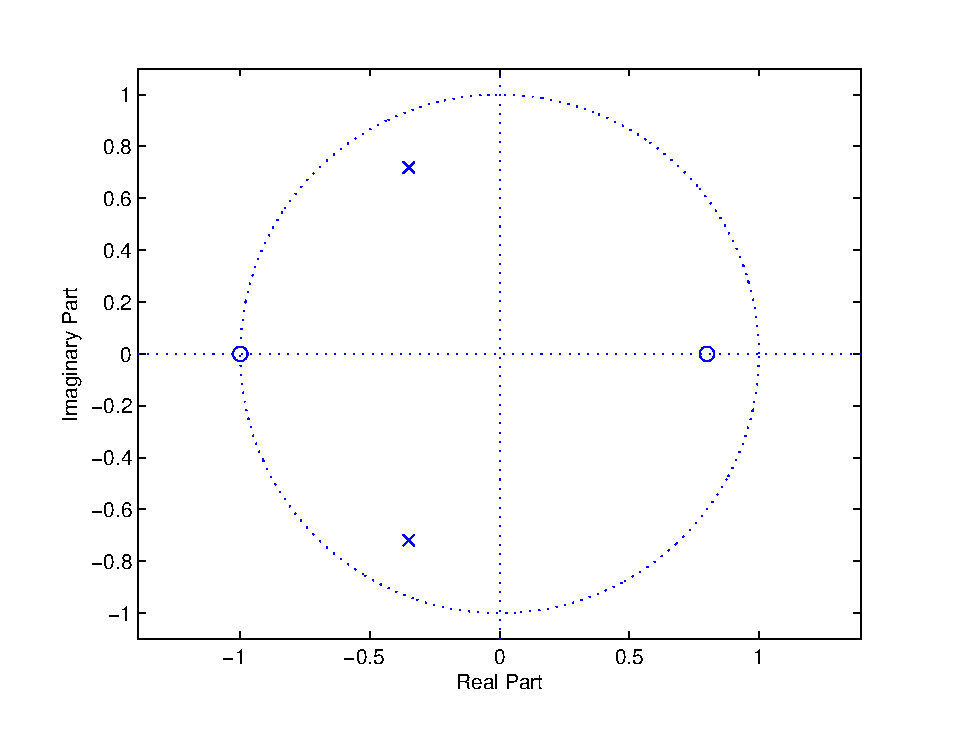
\includegraphics [width=3.0in]{polezero.eps}
		\caption{Pole-Zero Plot of H(z)}
		\label{fig:figure1}
	\end{center}
\end{figure}

\begin{par}
I then sketched the estimated frequency response from looking at the pole-zero plot.  This is included in Figure \ref{fig:figure2}.  I then compared this with MATLAB's output from the freqz command included in Figure \ref{fig:figure3}
\end{par}

\begin{figure}[htp]
	\begin{center}
		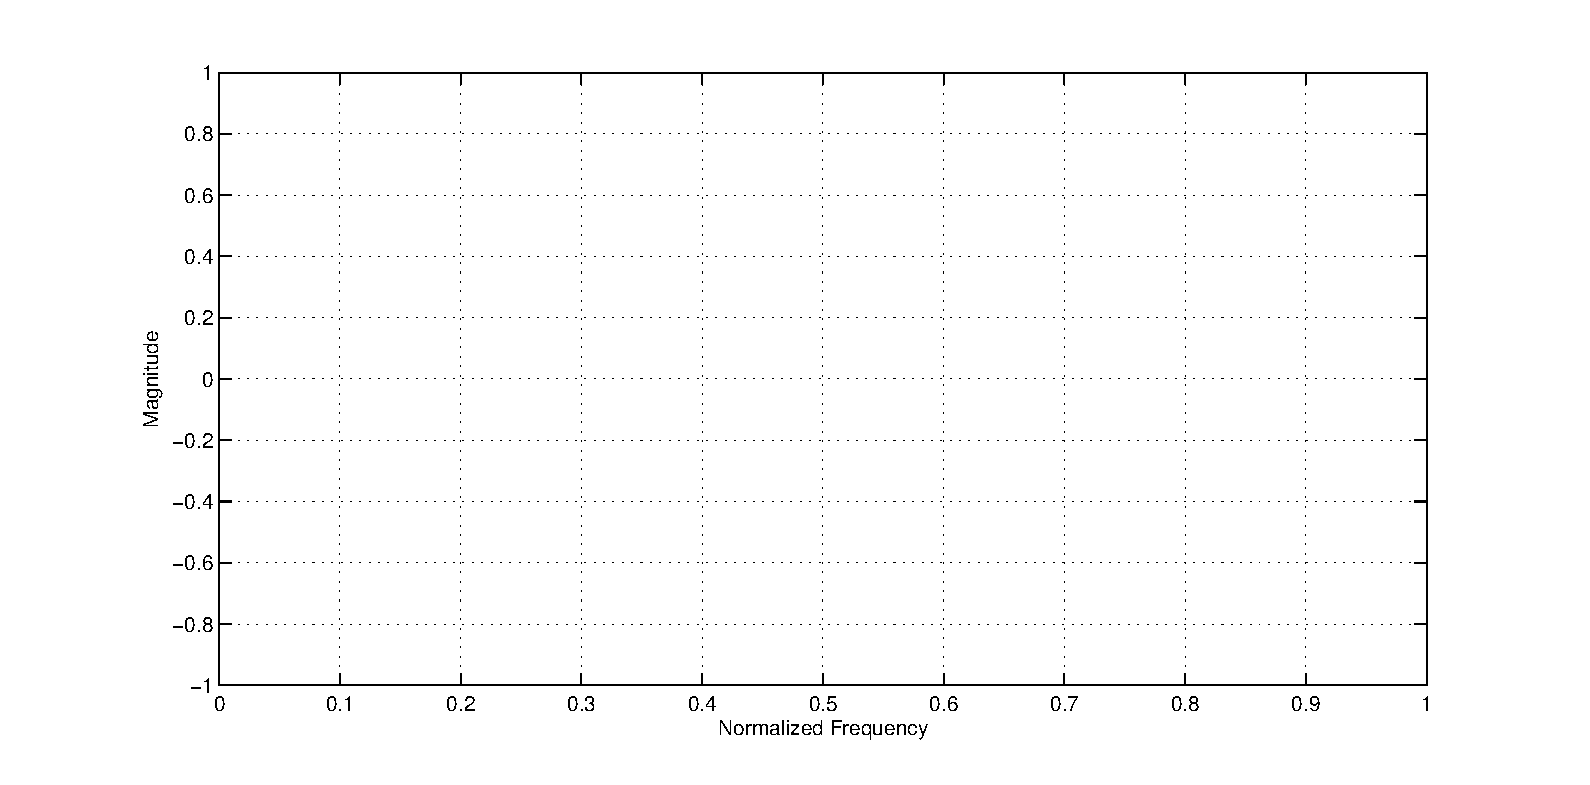
\includegraphics [width=6.0in]{sketch.eps}
		\caption{Sketched magnitude response of H(z)}
		\label{fig:figure2}
	\end{center}
\end{figure}

\begin{figure}[htp]
	\begin{center}
		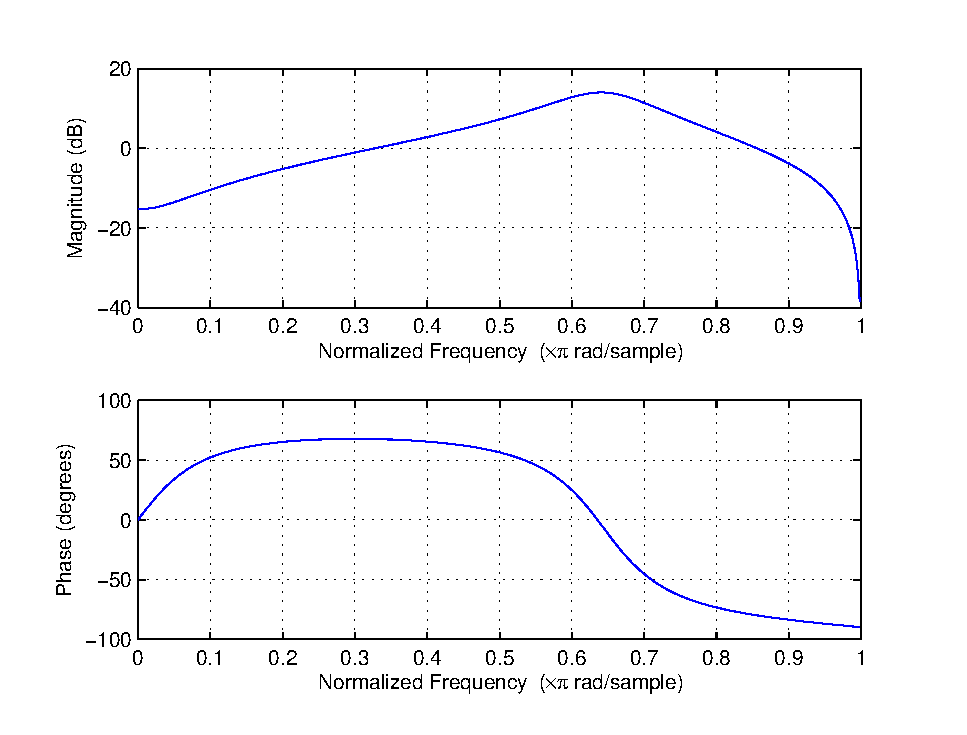
\includegraphics [width=6.0in]{freqz.eps}
		\caption{Frequency response of H(z)}
		\label{fig:figure3}
	\end{center}
\end{figure}

\section*{Question 2}
\begin{par}
I then used MATLAB's fdatool to design a high-pass filter.

The transfer function of my designed filter is:
$$HP(z) = \frac{1 - 1.957z^{-1} + 0.9571z^{-2}}{1 + 0.25z^{-2}}$$

The magnitude response plot is included in Figure \ref{fig:figure4} and the zero-pole plot is included in Figure \ref{fig:figure5}
\end{par}

\begin{figure}[htp]
	\begin{center}
		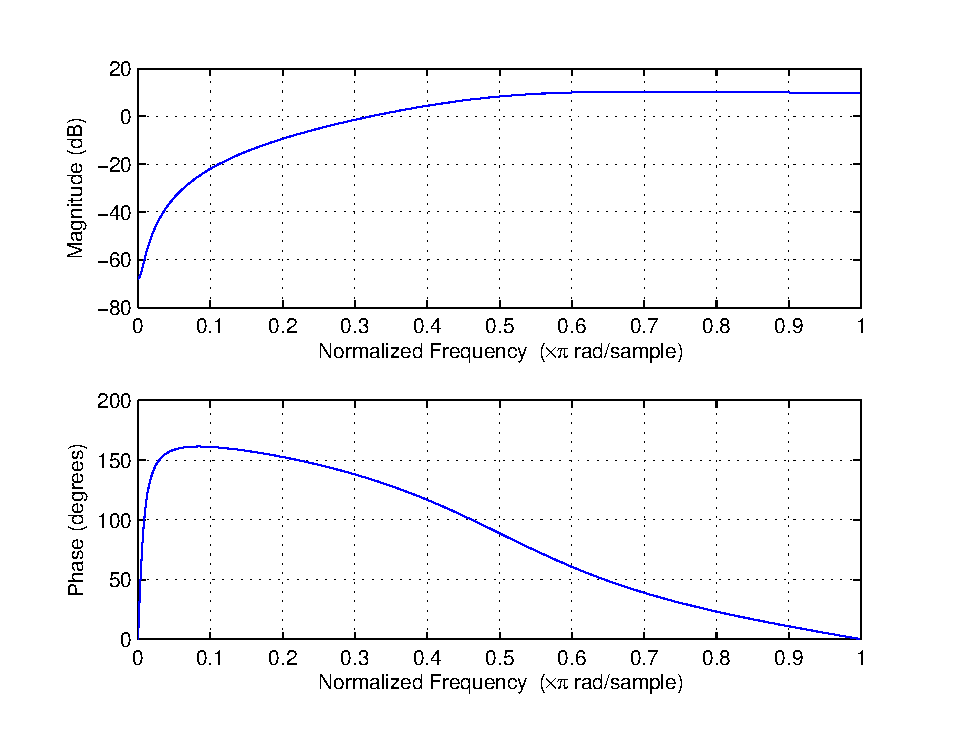
\includegraphics [width=3.0in]{hpmagresp.eps}
		\caption{fdatool high-pass filter magnitude response}
		\label{fig:figure4}
	\end{center}
\end{figure}

\begin{figure}[htp]
	\begin{center}
		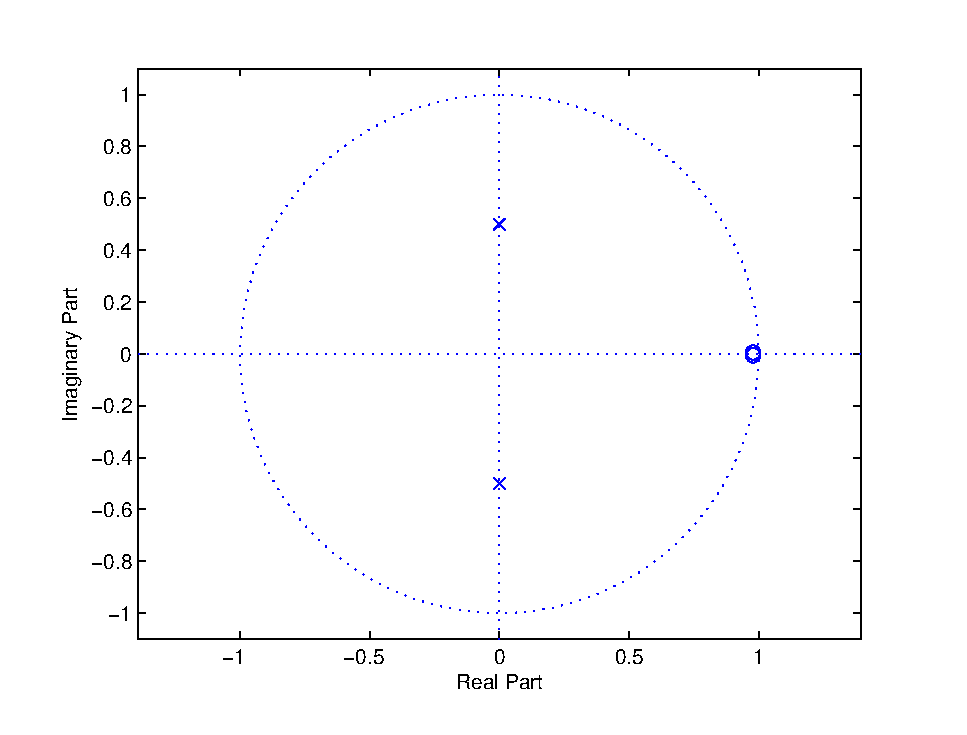
\includegraphics [width=3.0in]{hpzplane.eps}
		\caption{Pole-zero plot of fdatool high-pass filter}
		\label{fig:figure5}
	\end{center}
\end{figure}

\section*{Question 3}
\begin{par}
The difference equation for the filter is then:
$$y[n] = -0.25y[n-1] + x[n] - 1.957x[n-1] + 0.9571x[n-2]$$

To test the filter, I generated an input signal and used the filter command.  The results are in Figure \ref{fig:figure6}.  The filter that I created successfully attenuates the lower frequency.  It is not easy to tell directly from the output of the filter, but the results are reflected better in the FFT of the output.  I have included the FFT in Figure \ref{fig:fft}.  The lower frequency is clearly attenuated in the output of the filter.\\
\\
An interesting thing to note is that peaks appear in the output signal in places where there were no peaks in the input.  This may be due to the highly nonlinear phase response of the high-pass filter.
\end{par}

\begin{figure}[htp]
	\begin{center}
		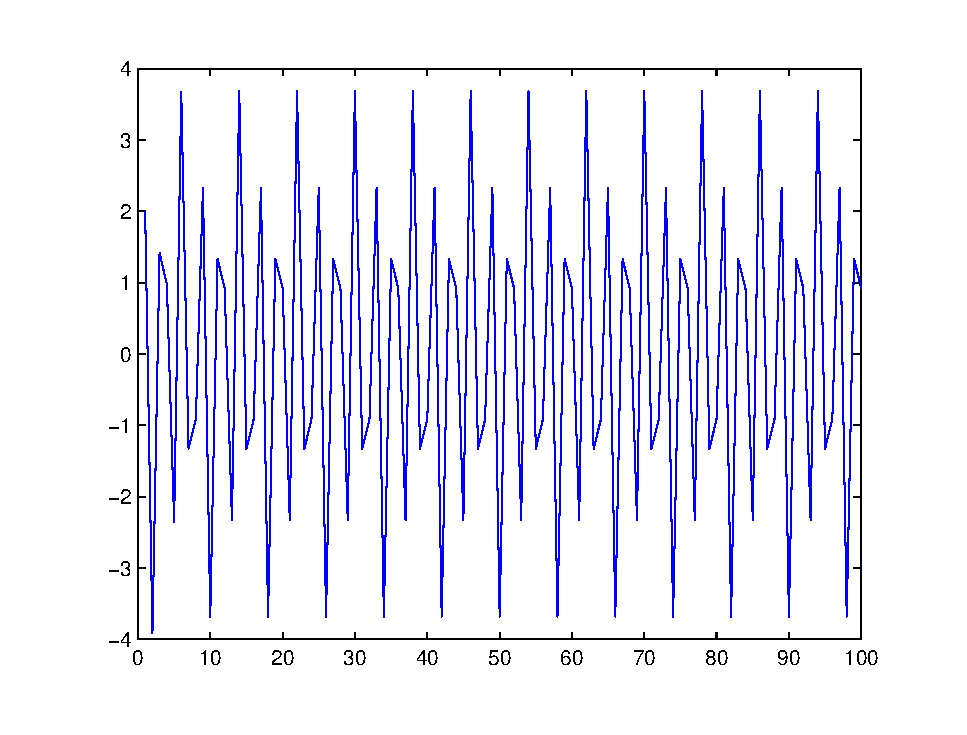
\includegraphics [width=3.0in]{filterresp.eps}
		\caption{Filter response to sinusoidal inputs}
		\label{fig:figure6}
	\end{center}
\end{figure}

\begin{figure}[htp]
	\begin{center}
		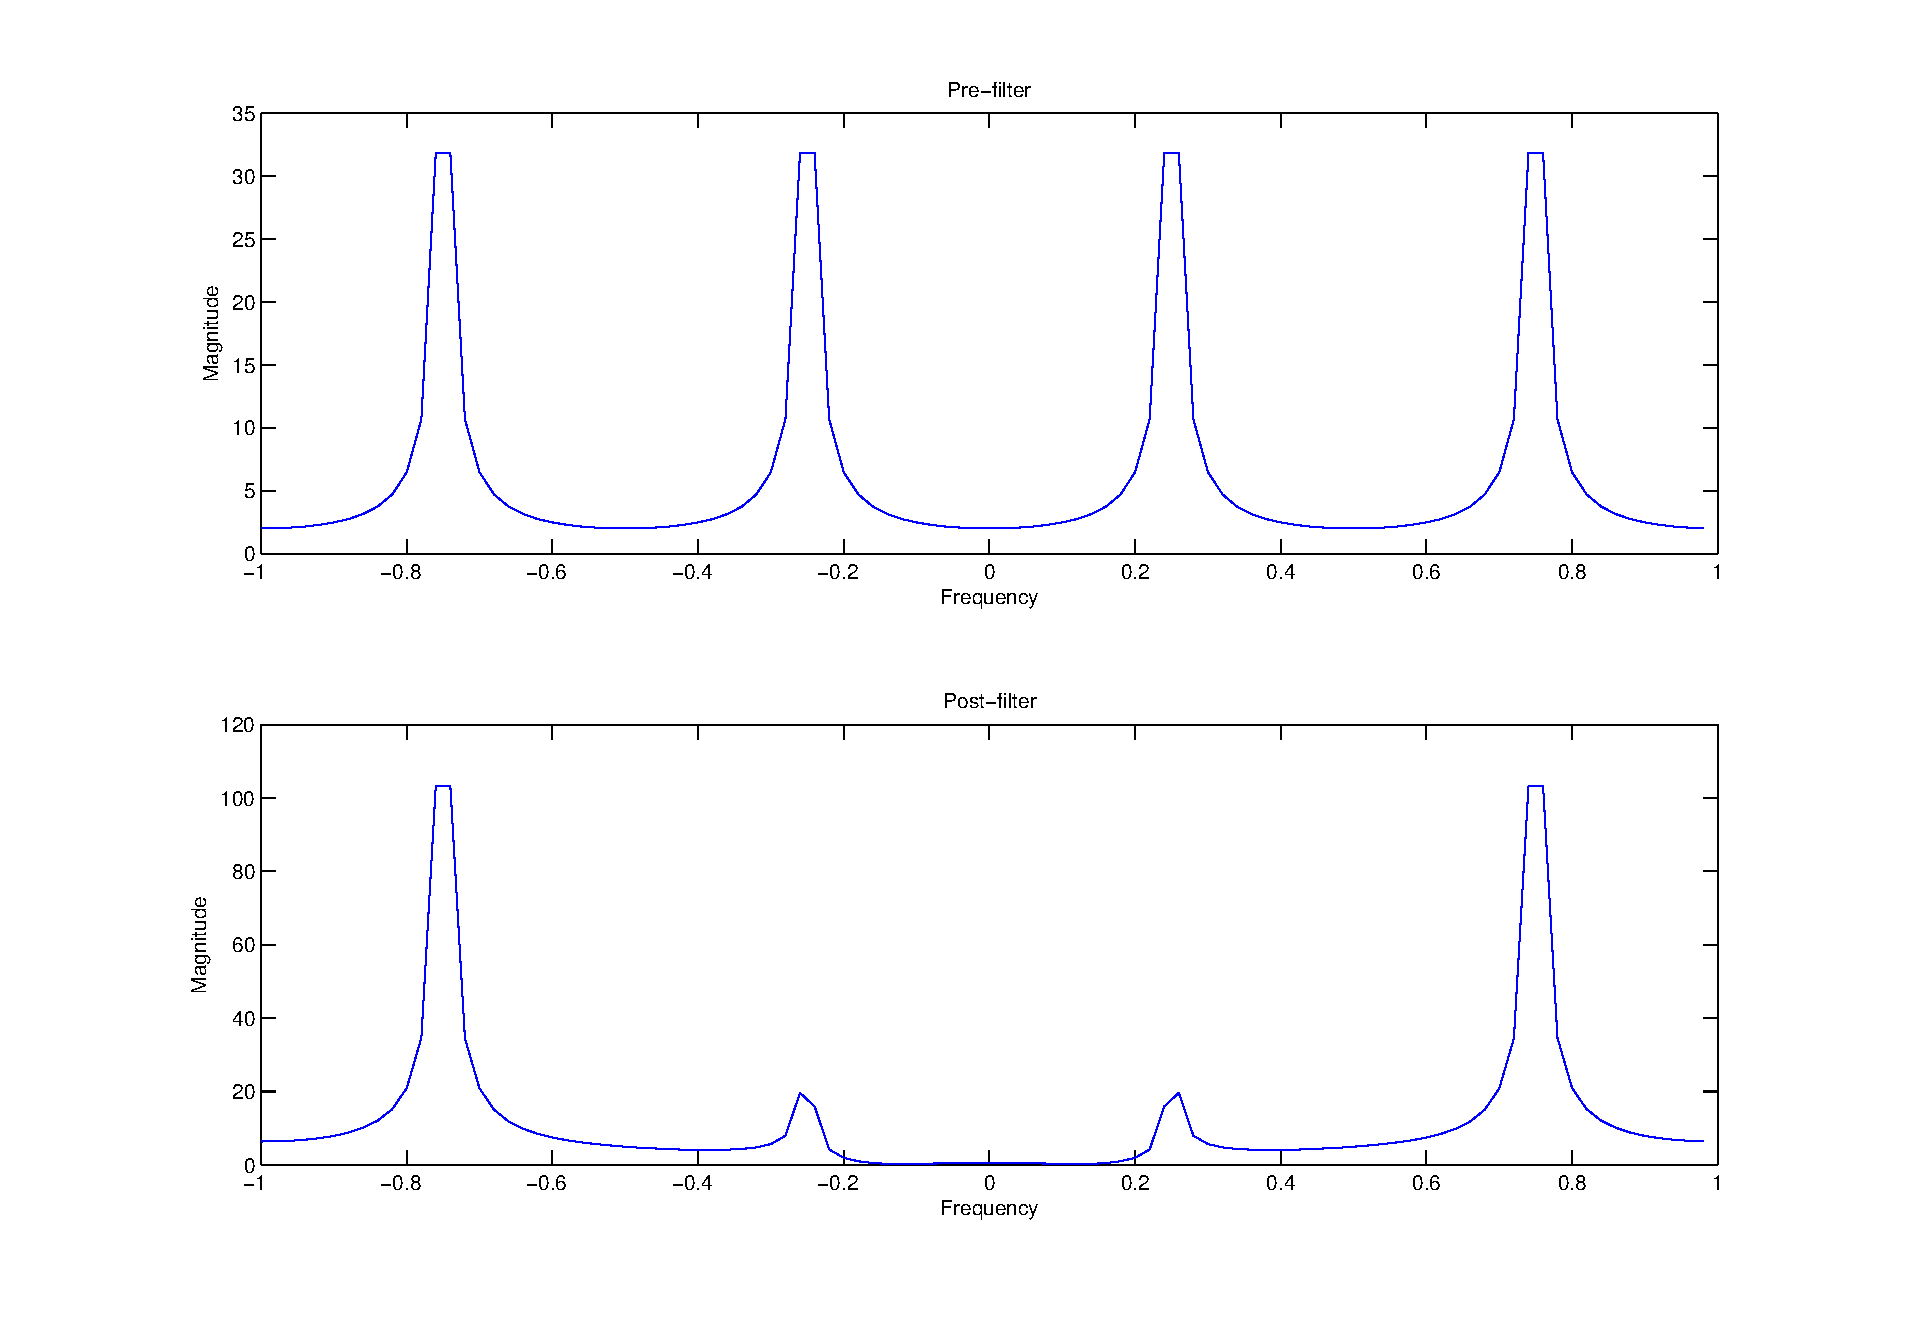
\includegraphics [width=3.0in]{fft.eps}
		\caption{FFT of filter output}
		\label{fig:fft}
	\end{center}
\end{figure}

\section*{Question 4}
\begin{par}
I then generated the impulse response of the high-pass filter.  It is included in Figure \ref{fig:figure7}.  \\
\\
The impulse response appears to be that of a high-pass filter.  A high-pass filter impulse response is characterized by a sharp "point" (or delta) at the origin, with negative samples around it.  When the impulse response is convolved with an input signal, the parts of the input signal with sharp changes (high-frequency regions) will be amplified, while those with wide, sweeping changes (low-frequency regions) will be attenuated.\\
\\
This is opposite of the impulse response of a low-pass function, which is characterized by a wide, sweeping appearance.  A low-pass filter would be ideally characterized by a wide pulse or a sinc function.
\end{par}

\begin{figure}[htp]
	\begin{center}
		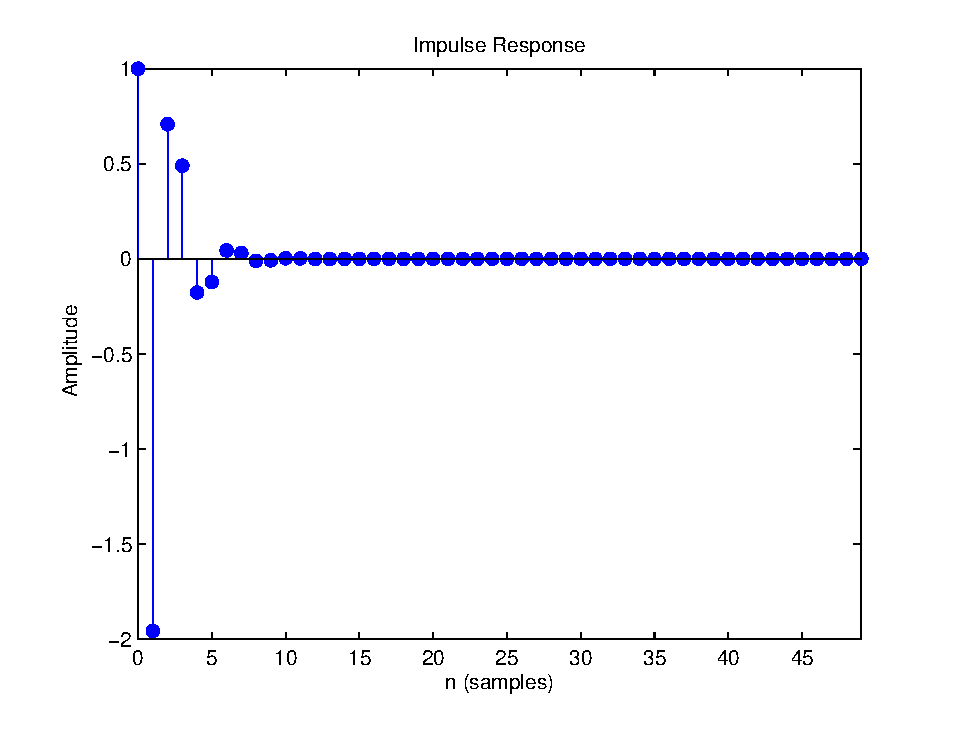
\includegraphics [width=3.0in]{impresp.eps}
		\caption{Impulse response of fdatool high-pass filter}
		\label{fig:figure7}
	\end{center}
\end{figure}

\section*{Question 5}
\begin{par}
I loaded the fanfare.au music sample into MATLAB.  The unfiltered file has a full range of audio, from bass notes to high notes.  Once passed through the filter, the song then becomes "tinny," and loses all of the low-end "punch."  This agrees with the fact that the lower frequencies have been filtered out of the song.
\end{par}
\begin{lstlisting}[language=matlab]
fanfare = auread('/Users/mjcarroll/Downloads/fanfare.au')
sound(fanfare)
sound(filter(HPnum,HPden,fanfare))
\end{lstlisting}

\end{document}

